\documentclass[a4paper,12pt,oneside,bibtotoc,numbers=noenddot]{scrreprt}

%Pakete
\usepackage[latin9]{inputenc}
\usepackage[ngerman]{babel}

\usepackage{listings}
\usepackage{graphicx}

%\usepackage{makeidx}
%\makeindex


\usepackage{BachelorThesis}

% Allgemeine Informationen
\newcommand\mytitle{Titel der Arbeit}
\newcommand\myauthor{Name des Autors oder der Autoren}
\newcommand\mydepartment{Informatik und Elektrotechnik}
\newcommand\myinstitute{Hochschule Zittau/G\"{o}rlitz}
\newcommand\mytutor{Name und Titel des betreuenden Professors}
\newcommand\mySecondTutor{Name und Titel des betrieblichen Betreuers}

% Abstracts
\newcommand\mysubject{Das deutsche Abstract.}
\newcommand\mysubjectenglish{The english abstract.}

% PDF-Einstellungen
\hypersetup
{
	pdftitle = \mytitle,
	pdfsubject = \mysubject,
	pdfauthor = \myauthor,
	pdfkeywords = {},
	colorlinks = {true},
	pdfborder = 0 0 0
}


\begin{document}
\nocite{*}


%
\pagenumbering{alph}
\begin{titlepage}
\thispagestyle{empty} 
 \begin{center}
 {\bfseries \LARGE Teil 1\\}
 {\bfseries \huge Das Wohnheimprojekt \\} 
 \vspace{1cm}
 {\bfseries \LARGE Teil 2\\}
 {\bfseries \huge Das Projekt Datenbankkonfigurationen\\}
 \vspace{1.0cm} 
 {\bfseries \huge Belegarbeit\\}
 \vspace{1.0cm}
 {\normalsize eingereicht als Entwurf am Fachbereich\\}
 {\bfseries \Large Informatik\\}
 {\normalsize der Hochschule Zittau/G�rlitz (HAW)\\}
 \vspace{1cm}
 {\normalsize als Pr�fungsleistung im Fach\\}
 {\bfseries \Large Fortgeschrittene Datenbank-Konzepte 1\\}
 \vspace{1cm}
 {\normalsize vorgelegt von:\\}
 {\bfseries \Large Christof Ochmann (35989)\\
 Stefan L�ttke (xxxxx) \\
 Ingo K�rner (40586)\\}
 \vspace{1cm}
 {\normalsize  G�rlitz, 27. Januar 2012\\}
 \vspace{0.5cm}
 Betreuer:	Prof. ten Hagen\\
 \vfill
\end{center}
\end{titlepage}

%

%% Kurzreferat
\thispagestyle{empty}
\section{Abstract}\label{Abstract}
Diese Arbeit besch�ftigt sich damit, wie sich die Performance von Abfragen steigern l�sst. Dabei wird nur der Bereich OLAP betrachtet. Der Datenimport mit Load sowie der Bereich OLTP werden nicht untersucht. Es wird nur auf Kaltstarts eingegangen, wie sie im Bereich Datawarehouse vorkommen. Performancesteigerungen mittels Caching bei Warmstarts sind nicht Gegenstand dieser Arbeit. Es wird untersucht, wie sich verschiedene Arten von Indexen und verschiedene Arten des Partitionings auf die Abfrageperformance von SQL-Queries auswirken. F�r die empirischen Messungen der Performance wird exemplarisch das Szenario eines Onlineshops gew�hlt, indem die Verk�ufe analysiert werden.\\
Diese Arbeit beantwortet die Frage, welche Datenbankkonfiguration f�r die gew�hl\-ten SQL-Abfragen im Durchschnitt die h�chste Abfrageperformance leistet. Ziel der Arbeit ist, Annahmen �ber die Performance verschiedener Konfigurationen zu treffen, diese theoretisch zu begr�nden und dann durch Messergebnisse praktisch zu belegen. Anhand von Messergebnissen werden die aufgestellten Hypothesen best�tigt oder wiederlegt. F�r wiederlegte Hypothesen wird eine Begr�ndung gesucht. Es wird davon ausgegangen, dass verschiedene Indexarten einen unterschiedlichen Einfluss auf bestimmte Queries haben werden. Es wird gezeigt, bei welchen Queries welche Indexarten bei welchen Spalten die Ausf�hrungszeit beschleunigen. Es wird angenommen, dass verschiedene Partitionierungsarten einen unterschiedlichen Einfluss auf bestimmte Queries haben werden. Es wird gezeigt, bei welchen Queries welche Partitionierungsarten auf welchen Spalten die Ausf�hrungszeit beschleunigen.\\
�ber die Ergebnisse der Arbeit l�sst sich zusammenfassend sagen, dass Hashindexe auf Prim�r- und Fremdschl�ssel die Abfragen im Durchschnitt um Faktor x beschleunigen, gegen�ber dem Weglassen s�mtlicher Indexe. Wird dar�ber hinaus X-Partitioning verwendet, beschleunigt das die Abfragen im Durchschnitt nochmal um Faktor x, gegen�ber der reinen Verwendung von Indexen. Wird dar�ber hinaus sogar ein Subpartitioning verwendet, beschleunigt das die gew�hlten Abfragen im Durchschnitt um Faktor x, gegen�ber der Verwendung von Partitions mit Indexen.

%\mysubject
%\section*{Abstract}
%\mysubjectenglish

\pagenumbering{Roman}
\tableofcontents
\listoffigures
\lstlistoflistings

\begin{listofacronyms}
\acronym{OLAP}{Online Analytical Processing}
\acronym{OLTP}{Online Transaction Processing}
\end{listofacronyms}

\begin{flushleft}
\begin{thebibliography}{sotief}
\bibitem{bib1}{Martin, Robert C. (2008): Clean Code: A Handbook of Agile Software Craftsmanship. Prentice Hall International}

\bibitem{bib2}{Freeman, Eric (2007): Entwurfsmuster von Kopf bis Fu�. O'REILLY}

\bibitem{bib3}{\begin{verbatim}http://www.easymock.org/EasyMock3_0_Documentation.html
Abruf (21.12.2011)\end{verbatim}} 

\bibitem{bib4}{\begin{verbatim}http://dev.mysql.com Abruf (11.01.2012)\end{verbatim}} 

\end{thebibliography}
\end{flushleft}



\newpage
\pagestyle{chapterStyle}
\pagenumbering{arabic}


\part{Wohnheimprojekt}

\part{Das Projekt Datenbank\-konfigura\-tionen}

\chapter{Theorie}
\section{Einleitung}\label{einleitung}
Ziel dieses Projektes ist die Performance eines relationalen Datenbankmagagementsystems f�r bestimmte Konfigurationen zu testen. Die Konfiguration ergibt sich aus den Anforderungen, die an das DBMS bzw. die konkrete Datenbank gestellt werden. 
Es ergibt sich die Frage, f�r welche konkrete Anforderung welche konkrete Konfiguration gew�hlt werden sollte? Um diese Frage zu beantworten, sind mehrere Schritte n�tig. Es wird zuerst ein DBMS exemplarisch ausgew�hlt. Dann wird f�r dieses DBMS ein ERD angefertigt, dass die Tabellen beschreibt. Um die Performance zu testen, muss ein Datengenerator geschrieben werden, der die Testdaten f�r die Tabellen generiert. Die konkreten Anforderungen, die an den Datengenerator gestellt werden, m�ssen analysiert werden. Dann wird der Generator entworfen, implementiert und getestet. F�r den Datengenerator wird ein Build Mangagement Tool eingesetzt sowie Frameworks f�r Dependency Injection und zum Testen der Anwendung. Dann werden f�r die Konfigurationen Queries auf den mit Testdaten bef�llten Tabellen gefahren und die Antwortzeiten gemessen. Die Messungen erfolgen alle auf einem Referenzsystem. So k�nnen verschiedene Konfigurationen �ber ihre Performancewerte miteinander verglichen werden.
\section{Aufgabenstellung}\label{Aufgabenstellung}
In diesem Projekt soll die Abfrage-Performace f�r ein bestimmtes Szenario gemessen werden. Dazu ist ein Szenario auszuw�hlen, das im Bereich OLAP und Data Warehouse angesiedelt ist. F�r das Szenario sind geeignete Konfigurationen zu w�hlen. Konfigurationen unterscheiden sich in Art- und Anzahl von Indexen und in den Partitionierungsarten. Es wird angenommen, dass jede Konfiguration f�r eine bestimmte Art von Abfragen besonders geeignet ist. Es sollen verschiedenartige Abfragen gew�hlt werden, f�r die jeweils die Performance gemessen wird. Um die Performance messen zu k�nnen, ist ein ERD f�r ein gew�hltes Szenario anzufertigen. Die Tabellen des ERD sollen mit Testdaten gef�llt werden. Dazu ist ein Datengenerator anzufertigen. Die Abfragen werden auf die gef�llten Tabellen angewendet. Die Zeit, die ein Query braucht, um auf einer bestimmten Konfiguration ausgef�hrt zu werden, wird gemessen. Das Messergebnis wird mit der Annahme verglichen und ausgewertet.
\section{Relevanz des Forschungsgegenstandes}\label{RelevanzDesForschungsgegenstandes}
Der Forschungsgegenstand in dieser Arbeit ist es, geeignete Konfigurationen f�r verschiedene, konkrete, praxisrelevante Anwendungsf�lle zu finden. \\
Der Forschungsgegenstand ist relevant, da bisher keine konkreten Werte, die die Performance der gew�hlten Konfigurationen beschreibt, vorliegen. Ziel dieser Foschung ist es, die Annahmen f�r Konfigurationen zu treffen, die Performance der Konfigurationen zu messen und dann zu interpretieren, ob die Annahmen sich mit den Messergebnissen best�tigen oder wiederlegt werden. Die Herausforderung dieser Arbeit ist, geeignete Anwendungsf�lle aus verschiedenen Anforderungen von Anwendungen zu finden. F�r jede dieser Anwendungsf�lle die geeignetste Kongiguration zu w�hlen. F�r diese Konfiguration werden dann Annahmen getroffen und Performancewerte gemessen. Die Annahmen werden dann mit Hilfe der Messergebnisse verifiziert bzw. falsifiziert. Um die Performance von Konfigurationen messen zu k�nnen, muss ein Testdatengenerator angefertigt werden. Dabei m�ssen technische Probleme gel�st werden. Um die optimale Konfiguration f�r einen Anwendungsfall zu finden, muss sich vertiefend in eine Datenbanken eingearbeitet werden. Das geschieht z.B. unter Zuhilfenahme von B�chern und Online-Ressourcen. In diesen Medien ist der Forschungsstand zur Erstellung von Konfigurationen dokumentiert.
\section{Der aktuelle Wissensstand}
Vorhandene Kenntnisse �ber die Erstellung von Konfigurationen werden haupt\-s�chlich aus Onlineressourcen bezogen. Bei der Umsetzung der Anforderungen wird aus mehreren L�sungsm�glichkeiten jeweils die am besten geeignete ausgew�hlt und die Wahl wird begr�ndet. Prim�rliteratur zur gew�hlten Datenbank ist unter www.XXX.de zu finden. Unter dieser Adresse ist das gew�hlte DBMS dokumentiert. Auf dieser Seite wird eine Einf�hrung in XXX gegeben. Es gibt Installationsanleitungen, Programmier-Tutorials, eine umfassende Dokumentation von XXX und Werkzeuge die ein effizienteres Arbeiten mit XXX erm�glichen.
\section{Anwendungsf�lle f�r Datenbankanwendungen}\label{AnwendungsfaelleFuerDatenbankanwendungen}

\begin{itemize}
\item \textbf{Anwendungsfall 1}\\
Ein Online-Shop will seine Bestellungen �ber eine MySQL-Datenbank abwickeln. (innoDB)

\item \textbf{Anwendungsfall 2}\\
Das Management des Online-Shops m�chte Abfragen auf bestimmten Tabellen t�tigen, wie z.B.:

\begin{itemize}
\item Welches Produkt wurde wie oft gekauft?
\item Wieviel Umsatz wurde von wem in einem bestimmtem Zeitraum generiert?
\item Wie viele Kunden haben in einem bestimmten Zeitraum bestellt?
\end{itemize}

Dabei soll die Antwortzeit auch bei Queries �ber alle Daten nicht l�nger als eine Sekunde dauern. (Memory)

\item \textbf{Anwendungsfall 3}\\
Ein bekannter Blogger m�chte das Weblog-System WordPress einsetzen um Beitr�ge zu ver�ffentlichen. Die Kommentare und Blog-Posts werden strukturiert gespeichert. Zu bestimmten Spitzenzeiten laden hunderte Leser gleichzeitig seine Blogposts. (MyISAM)

\item \textbf{Anwendungsfall 4}\\
In einer Erdbebenwarnstation sollen Bodenersch�tterungen durch einen Seismografen erfasst und digital archiviert werden. Der Seismograf misst 50 mal in der Sekunde. Es sollen auch feinste Amplitudenausschl�ge erfasst werden. (Archive)
\end{itemize}
\subsection{EasyMock}
EasyMock 3.0 ist ein Test-Framework zur dynamischen Generierung von Mock Objekten f�r Schnittstellen und Klassen. Mock-Objekte werden f�r Unit-Tests von Java-Programmen verwendet.

\subsubsection{Was ist ein Mock-Objekt?}
Beim Unit-Testing kollaborieren Units mit anderen Units. Die Kollaborateure werden durch Mock Objekte simuliert. Im Gegensatz zu einem Stub �berpr�ft das Mock-Objekt, ob es wie erwartet verwendet wurde. In einem Unit-Test werden Klassen bzw. Methoden isoliert von ihrer Umgebung getestet. Um die Testobjekte isoliert zu testen, m�ssen die Schnittstellen des Testobjekts durch Mock-Objekte ersetzt werden. Die Mock-Objekte sind Platzhalter f�r die echten Objekte. Das Verhalten eines dynamischen Mock-Objekts wird nicht in einer Klasse programmiert, sondern von dem Unit-Test aufgezeichnet. Es m�ssen keine Klassen von Hand geschrieben werden. Es muss auch kein Quellcode der Mock-Klassen, mit den echten Klassen synchron gehalten werden. Mock-Objekte werden bei EasyMock ''on the fly'' generiert, sind sicherer gegen Refactoring und damit besonders f�r Test Driven Development geeignet.

\subsubsection{Wie wird EasyMock benutzt?}
Um EasyMock zu benutzen, sind folgende Schritte n�tig:
\begin{enumerate}
	\item das Mock-Objekt von der Klasse / Schnittstelle die simuliert werden soll, erzeugen und dem zu testenden Objekt �bergeben,
	\item das erwartete Verhalten aufzeichnen,
	\item das Mock-Objekt auf Wiedergabe-Modus stellen,
	\item verifizieren, ob das Mock-Objekt auch so benutzt wurde, wie in Schritt zwei spezifiziert
\end{enumerate}
\subsection{Dependency Injection}
Um Abh�ngigkeiten zwischen Objekten zu minimieren, wird das Architektur-Muster Dependency Injection verwendet. Dabei k�mmert sich das Objekt nicht mehr selbst um die Erzeugung seiner abh�ngigen Objekte. Diese Abh�ngigkeiten werden von einem Framework erstellt. Der Code des Objektes wird unabh�ngig von seiner Umgebung. Dadurch wird das Objekt leichter unit-testbar, da Abh�ngigkeiten zentral verf�gbar sind.

\subsubsection{Dependency Injection mit Google Guice}
F�r die Anwendung wird das Dependency Injection Framework Google Guice verwendet. Eine Abh�ngigkeit wird am besten �ber einen Konstruktor in ein Objekt injiziert. Daf�r braucht der Konstruktor nur mit @Inject annotiert werden.

Codebeispiel
\chapter{Datengenerator}\label{Datengenerator}
Die Testdaten zum F�llen der Tabellen werden mit einem Datengenerator erzeugt.

\section{Analyse}
Der Datengenerator soll die Testdaten f�r die vier Tabellen 
\begin{itemize}
	\item Kunde,
	\item Produkt,
	\item Warenkorb,
	\item WarenkorbProdukt
\end{itemize}
erzeugen und in die Tabellen schreiben. Dabei sollen dem Generator vier Parameter beim Start �bergeben werden:
\begin{enumerate}
	\item die Anzahl der zu erzeugenden Kunden
	\item die Anzahl der zu erzeugenden Produkte
	\item die Anzahl der Warenk�rbe pro Kunde
	\item die Anzahl der Produkte im Warenkorb
\end{enumerate}

Der Generator muss f�r alle beliebigen Startparameter die Tupel der einzelnen Tabellen korrekt miteinander verkn�pfen. Deswegen erzeugt der Generator auch die Prim�r- und Fremdschl�ssel der Tupel selbst. 
Die maximale Anzahl der Warenk�rbe ergibt sich aus der Anzahl der Kunden * der Anzahl der Warenk�rbe pro Kunde. In der Warenkorbtabelle m�ssen bei einer Anzahl von z.B. 10 Warenk�rben pro Kunde auch je 10 Warenk�rbe existieren, die mit ihrem Fremdschl�ssel auf den jeweiligen Kunden zeigen. In der Warenkorbtabelle sollen im Datum alle Monate des Jahres 2011 gleichm��ig verteilt vorkommen. 

Die maximale Anzahl der Bestellzeilen ergibt sich aus der Anzahl der Kunden * der Anzahl der Warenk�rbe pro Kunde * der Anzahl der Produkte in einem Warenkorb. Die m�glichen Produkte sollen gleichm��ig �ber alle Bestellzeilen verteilt sein. In der WarenkorbProdukt-Tabelle m�ssen bei einer Anzahl von z.B. 7 Produkten im Warenkorb auch je 7 Bestellzeilen existieren, die mit ihrem Fremdschl�ssel auf den jeweiligen Warenkorb zeigen.

F�r jede Tabelle soll ausgegeben werden, wieviel Zeit der Generator insgesamt f�r den Schreibvorgang ben�tigte. Damit wird es auch m�glich, die Schreibperformance einer Datenbankkonfiguration zu messen und auszuwerten.

\subsection{Anwendungsfalldiagramm}

Die Abbildung \ref{fig:AnwendungsfalldiagrammDatengenerator} auf Seite \pageref{fig:AnwendungsfalldiagrammDatengenerator} zeigt das Anwendungsfalldiagramm des Prototypen.

\subsection{User Stories}

1. AF - Datengenerator mit Aufrufparametern ausf�hren
Um die Testdaten zu generieren und in die Tabellen zu schreiben ruft der Anwender den Datengenerator als Jar-Datei �ber die Kommandozeile auf und �bergibt ihm die folgenden vier Aufrufparameter in gegebeneer Reihenfolge:
\begin{enumerate}
	\item die Anzahl der zu erzeugenden Kunden
	\item die Anzahl der zu erzeugenden Produkte
	\item die Anzahl der Warenk�rbe pro Kunde
	\item die Anzahl der Produkte im Warenkorb
\end{enumerate}

2. AF - Zeiten f�r die Schreibvorg�nge �bernehmen
Der Anwender notiert sich die vom Generator auf der Konsole ausgegebenen Gesamtzeiten der einzelnen Schreibvorg�nge.

3. AF - Anzahl der insgesamt geschriebenen Tupel pro Tabelle �bernehmen
Der Anwender notiert sich die auf der Konsole ausgegebenen Werte der vom Generator insgesamt geschriebenen Tupel f�r jede Tabelle.

\subsection{Nichtfunktionale Anforderungen}
Da im sp�teren Projektverlauf leicht neue Tabellen hinzukommen k�nnen, soll die Anwendung leicht anpassbar sein.

\subsection{Analyseklassendiagramm}
Die Abbildung \ref{fig:AnalyseDatengenerator} auf Seite \pageref{fig:AnalyseDatengenerator} zeigt das Analyseklassendiagramm des Datengenerators.

\subsection{UI-Mockup}
Die Abbildung \ref{fig:UI-MockUp} auf Seite \pageref{fig:UI-MockUp} zeigt das UI-Mockup des Datengenerators.



\begin{figure}[htp]
\centering
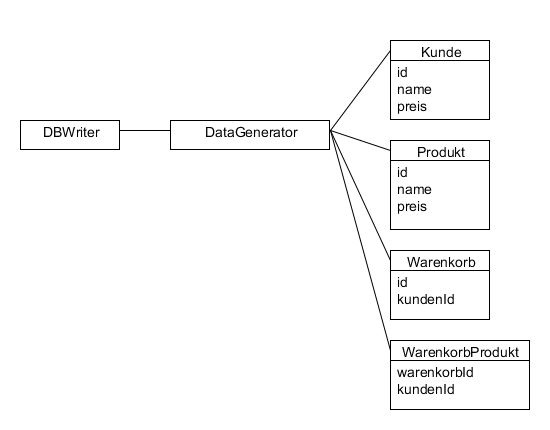
\includegraphics[width=0.8\textwidth]{Ingo/Bilder/AnalyseDatengenerator.png}
\caption{Analyse Datengenerator}
\label{fig:AnalyseDatengenerator}
\end{figure}

\begin{figure}[htp]
\centering
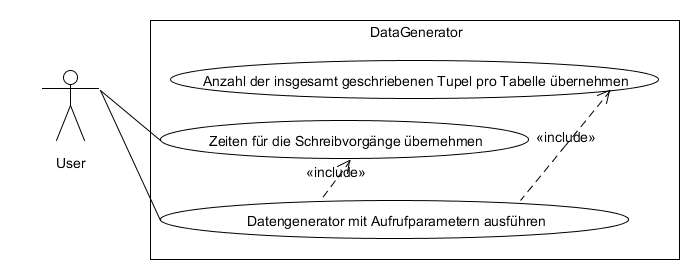
\includegraphics[width=0.8\textwidth]{Ingo/Bilder/AnwendungsfalldiagrammDatengenerator.png}
\caption{Anwendungsfalldiagramm Datengenerator}
\label{fig:AnwendungsfalldiagrammDatengenerator}
\end{figure}


\begin{figure}[htp]
\centering
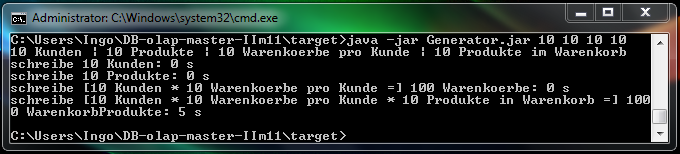
\includegraphics[width=0.8\textwidth]{Ingo/Bilder/UIMockUp.png}
\caption{UI-MockUp}
\label{fig:UI-MockUp}
\end{figure}
\section{Entwurf}
\subsection{Komponentendiagramm}
Abbildung \ref{fig:Komponentendiagramm} auf Seite \pageref{fig:Komponentendiagramm} zeigt das Komponentendiagramm.

\begin{figure}[htp]
\centering
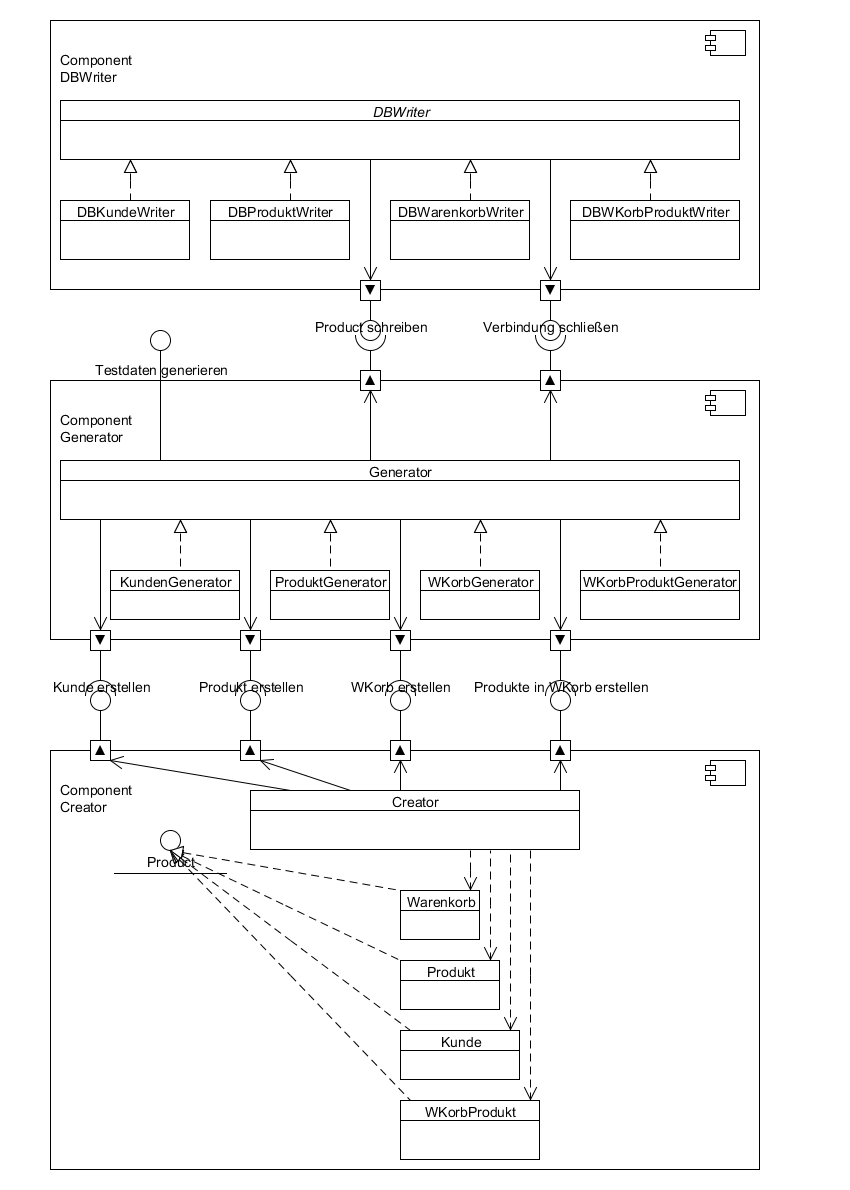
\includegraphics[width=0.8\textwidth]{Ingo/Bilder/Komponentendiagramm.png}
\caption{Komponentendiagramm}
\label{fig:Komponentendiagramm}
\end{figure}

\subsection{Entwurfsklassendiagramm der Generatorkomponente}
Abbildung \ref{fig:EntwurfGeneratorkomponente} auf Seite \pageref{fig:EntwurfGeneratorkomponente} zeigt das Entwurfsklassendiagramm der Generatorkomponente.

\begin{figure}[htp]
\centering
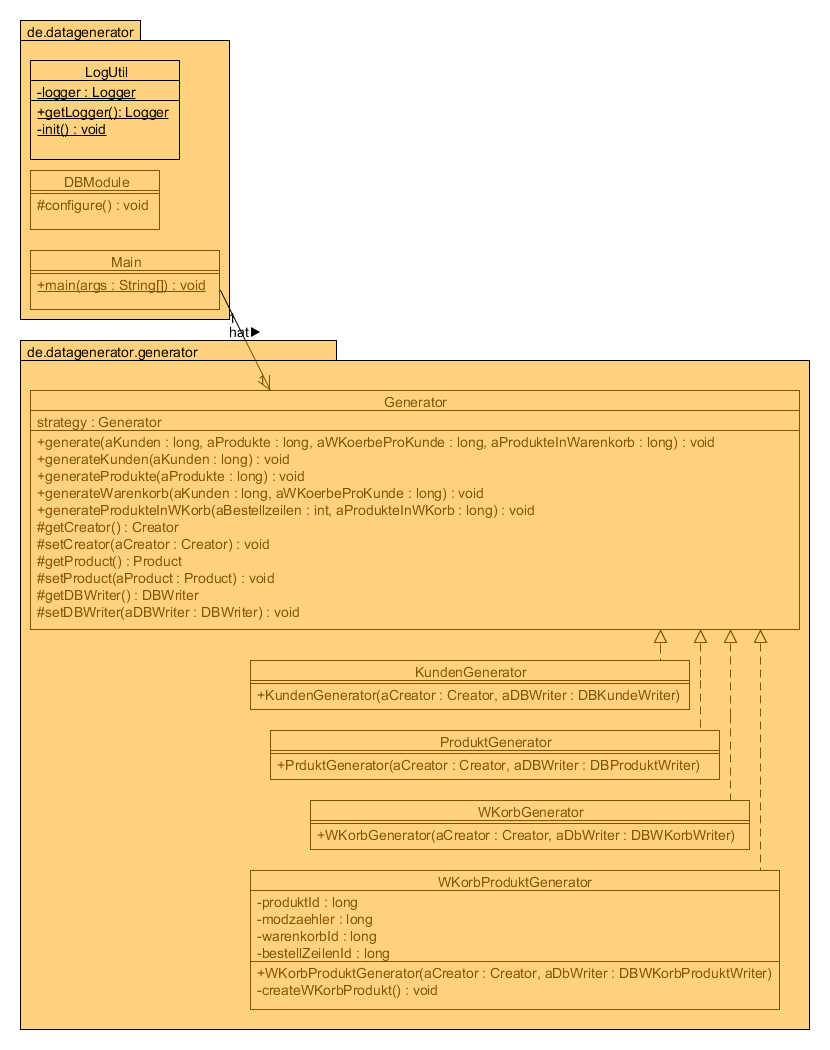
\includegraphics[width=0.8\textwidth]{Ingo/Bilder/EntwurfGeneratorkomponente.png}
\caption{Entwurf der Generatorkomponente}
\label{fig:EntwurfGeneratorkomponente}
\end{figure}

\subsection{Entwurfsklassendiagramm der DBWriterkomponente}
Abbildung \ref{fig:EntwurfDBWriterkomponente} auf Seite \pageref{fig:EntwurfDBWriterkomponente} zeigt das Entwurfsklassendiagramm der DBWriterkomponente.

\begin{figure}[htp]
\centering
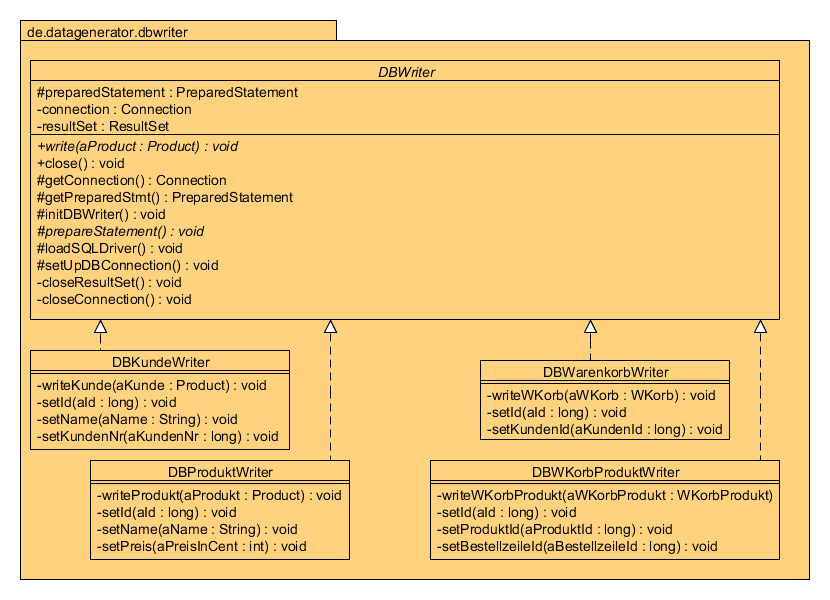
\includegraphics[width=0.8\textwidth]{Ingo/Bilder/EntwurfDBWriterkomponente.png}
\caption{Entwurf der DBWriterkomponente}
\label{fig:EntwurfDBWriterkomponente}
\end{figure}

\subsection{Entwurfsklassendiagramm der Creatorkomponente samt Datamodel}
Abbildung \ref{fig:EntwurfCreatorUndDatamodelKomponente} auf Seite \pageref{fig:EntwurfCreatorUndDatamodelKomponente} zeigt das Entwurfsklassendiagramm der Creatorkomponente und dem dazugeh�rigen Datamodel.

\begin{figure}[htp]
\centering
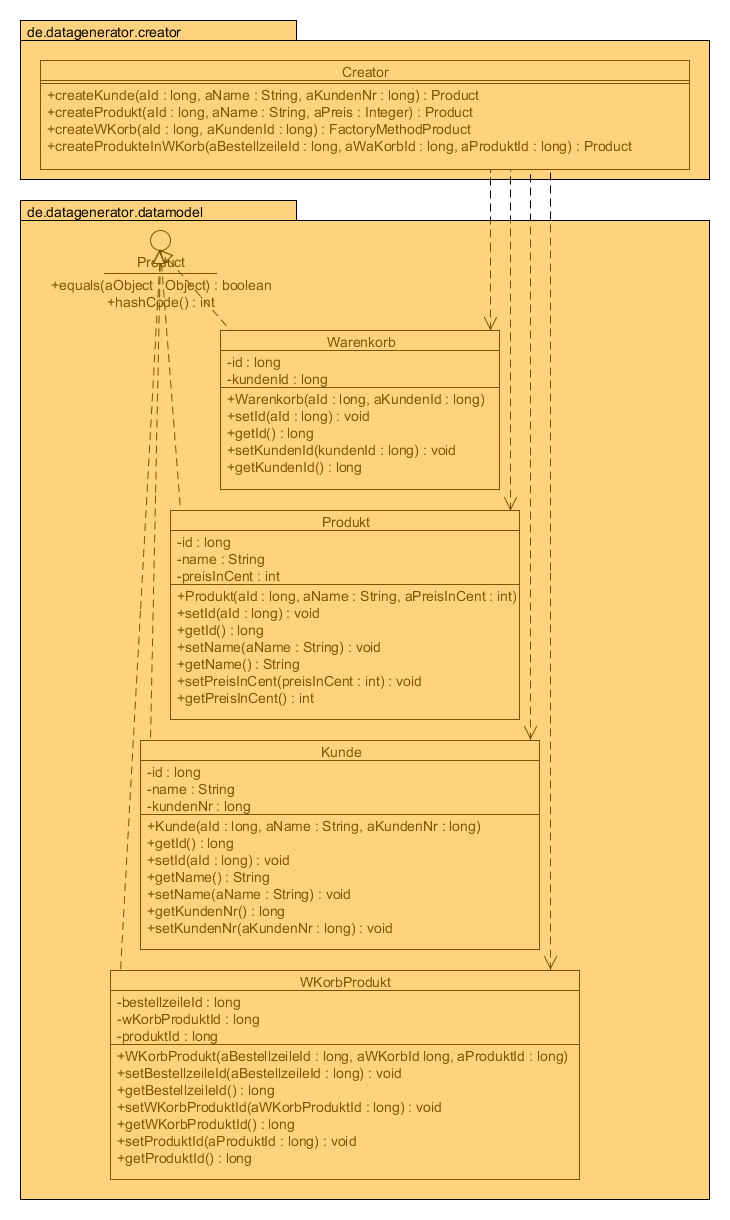
\includegraphics[width=0.8\textwidth]{Ingo/Bilder/EntwurfCreatorUndDatamodelKomponente.png}
\caption{Entwurf der Creatorkomponente}
\label{fig:EntwurfCreatorUndDatamodelKomponente}
\end{figure}

\subsection{Stored Procedures}
Der Generator hat eine zweischichtige Architektur (two tier architecture). Die Komponente Generator greift auf die Dienste der Komponente DBWriter zu. Auch sonst wurde in der Anwendung auf geringe Kopplung geachtet (demeters law).

\subsection{Prepared Statement}
Die generierten Testdaten werden �ber sogenannte Prepared Statements in die Tabellen geschrieben. Prepared Statements enthalten Platzhalter f�r die eigentlich zu schreibenden Daten. Prepared Statements bieten sich u.a. dann an, wenn sich bei dem Statement nur die Parameterwerte unterscheiden. Prepared Statements bringen einen Geschwindigkeitsvorteil, da sie bereits im DBMS vor�bersetzt werden und der DBWriter mit sehr viel generierten Parameterwerten aufgerufen wird.

\subsection{Entwurfsmuster}
Der Creator ist als einfache Fabrik implementiert. Durch ihn werden konkrete Instanziierungen aus dem Clientcode entfernt und somit die Clients von konkreten Klassen entkoppelt (Dependency Inversion Principle)

In z.B. DBWriter konnte initDBWriter() als Template Method implementiert werden. Sie definiert die Schritte f�r die Initialisierung eines DBWriters, wobei die Unterklassen entscheiden, wie sie die abstrakte Hook-Methode prepareStatement() implementieren. Durch die Template Method werden die Highlevel Komponenten loadSQLDriver() und setUpDBConnection() von Lowlevel Komponente prepareStatement() entkoppelt. Die Lowlevel-Komponenten prepareStatement() kann sich in ein System reinh�ngen, und Highlevel Komponenten bestimmen, wann und wie sie erforderlich sind. Die Lowlevel Komponente prepareStatement() ruft Highlevel Komponente nie direkt auf (Hollywood Prinzip).

\subsection{Implementierung und Test}
Das Projekt liegt als Maven-Eclipse-Projekt unter git@github.com:rinkdotrink/DB-olap-master-IIm11.git

\subsubsection{Projektumgebung}
Eclipse-IDE 3.7, JDK 1.7, JUnit 4.8.2, Maven 3, Guice 3, EasyMock 3.0, Log4J 1.2.16, mysql-connector-java 5.1.6, Umlet 11.3

\subsubsection{Projekt aus dem repository laden}
Berechtigungen
git pull

\subsubsection{Maven}

\subsubsection{Maven-Projekt in Eclipse importieren}



\subsubsection{Maven Projekt ausf�hren}
Entweder �ber Jar oder �ber Eclipse

\subsubsection{Jar mit allen Abh�ngigkeiten erstellen}
package


\subsection{Implementierung der Funktionalit�t}
Die drei Komponenten

\subsection{Unit Test mit EasyMock 3.0}


%\chapter{Theoretische Grundlagen}
%Die f\"{u}r den Untersuchungsgegenstand relevanten Themen, die \"{u}ber die
%grundlegenden Studieninhalte hinausgehen; oft auch anwendungsspezifische Aspekte - %ca. 6 Seiten

%\chapter{Ist-Analyse}
%Welche Defizite sollen mit der Arbeit behoben werden, welche nicht? %Pr\"{a}zisierung
%der Zielstellung - ca. 6 Seiten

%\chapter{L\"{o}sungskonzept}
%Wie sollen die Defizite behoben werden? Methoden, fachliche Auseinandersetzung
%mit alternativen Ans\"{a}tzen und Auffassungen, Systembeschreibung (Architektur,
%Vorgehensmodell, \ldots) - ca. 12 Seiten

%\chapter{Implementierung}
%Umsetzung des L\"{o}sungskonzepts, Begr\"{u}ndung der verwendeten Technologien - %ca. 8
%Seiten

%\chapter{Ergebnisse}
%Objektive Bewertung der vorliegenden L\"{o}sung, diverse Testverfahren,
%Nutzerbefragungen - ca. 4 Seiten

%\chapter{Fazit und Ausblick}
%Zusammenfassung s\"{a}mtlicher Ergebnisse in Bezug auf die Zielerf\"{u}llung und
%Vorschl\"{a}ge f\"{u}r weiterf\"{u}hrende Arbeiten - ca. 2 Seiten

\bibliographystyle{alphadin}
%\bibliography{literatur}

%\begin{appendix}
%\pagestyle{appendixAStyle}
%\chapter{Codebeispiele}

%\pagestyle{appendixBStyle}
%\chapter{Abbildungen}
%\end{appendix}


\newpage
\chapter{Arbeitsaufteilung}
\begin{table}[h]

	\begin{center}
		\begin{tabular}{|l||c|c|c|c|c|c|}
	  	\hline
	  		 \textbf{Arbeit}		&	\textbf{Cristof Ochmann}	&	\textbf{Stefan L�ttke}	& \textbf{Ingo K�rner}  \\ \hline \hline
				  			Abstract   	&                   &                   & ~\ref{Abstract}          \\
				  			Einleitung  &                   &          		      & ~\ref{Einleitung} 	             			\\
							  Aufgabenstellung&               &                   & ~\ref{Aufgabenstellung}     			            \\ 
							  Forschungsgegenstand&           &                   & ~\ref{RelevanzDesForschungsgegenstandes} \\ 
							  akt. Wissensstand&                   &                   & ~\ref{DerAktuelleWissensstand}  \\ 
							  Anwendungsf�lle&                &                   & ~\ref{AnwendungsfaelleFuerDatenbankanwendungen}\\ 
							  EasyMock   	&                   &                   & ~\ref{EasyMock} 			            \\ 
							  Dependency Injection&           &                   & ~\ref{DependencyInjection}     \\ 
							  Datengenerator&                 &                   & ~\ref{Datengenerator}         \\
							  \hline			  
			  	\hline
		\end{tabular}			
	\end{center}
\end{table}





%\baeiderkl{\myauthor}{G\"{o}rlitz, \today}
\newpage
\chapter{Eigenst�ndigkeitserkl�rung}
Hiermit erkl�re ich, dass ich diese Arbeit selbst�ndig verfasst habe. Mir ist bekannt, dass jede Form des Plagiats mit der Note 5 (Betrugsversuch) bewertet wird.

%\begin{tabular}{@{}llr@{}}
\begin{tabular}{@{}p{6.0cm}p{6.0cm}}
	  	
	  		 	
	  		 & \\
	  		 & \\
				  			\textbf{Ochmann, Christof} &               Unterschrift:\\		
				 &\\
				 & \\			
				  			\textbf{L�ttke, Stefan}   	&                   Unterschrift:\\			
				 &\\
				 & \\
				  			\textbf{K�rner, Ingo}   	&                     Unterschrift:\\
			
\end{tabular}


\end{document}
